%!TEX root = ../report.tex

\section{Ausdauer}
Definition: Ermüdungswiderstandsfähigkeit (konditionell und informationell) und Regenerationsfähigkeit

\subsection{Systematik}
\subsubsection{Belastungsdauer}
\begin{itemize}
  \item Kurzzeitausdauer (<35s)
  \item Mittelzeit-Ausdauer(35s - 8min)
  \item Langzeitausdauer (> 8min): LZA I: 8-30min, LZA II: 30min - 3h, LZA III: 3-9h, LZA IV: >9h
\end{itemize}

\subsubsection{Allgemeine vs spezielle Ausdauer}
\begin{itemize}
  \item Allgemeine Ausdauer: Grundlage für Regeneration, Training und Erholung und Voraussetzung für spezielles Training
  \item Spezielle Ausdauer: Wettkampfspezifische Ausdauer-Anforderungen (wichtiger für sportlichen Erfolg)
\end{itemize}

\paragraph{KsA: Koeffizient der speziellen Ausdauer}
= durchschnittliche 100m-Zeit obere Nachbarstrecke / durchschnittliche 100m-Zeit untere Nachbarstrecke

\subsection{Energiebereitstellung}
\paragraph{Mechanismen}
\begin{itemize}
  \item Systematik: Je nach Dauer und Intensität der Belastung wird Energie aus verschiedenen Substanzen gewonnen.
  \item Energiegewinnung aus Substrat:
    \begin{itemize}
      \item Energiefluss: Rate, mit der Energie zur Verfügung gestellt werden kann.
      \item Kapazität: Energievorrat
    \end{itemize}
  \item Problem: Maximale Energie nur kurzfristig verfügbar\\
    Dauerleistungsgrenze: ca 40%
  \item Energiearten
    \begin{itemize}
      \item alaktazid (Cache (high transfer, low capacity))
      \item laktazid (Memory)
      \item aerob (Drive)
    \end{itemize}
\end{itemize}

\subsection{Determinaten der Ausdauer}
\begin{centering}
\begin{tabular}{m{0.2\textwidth} | m{0.3\textwidth} | m{0.3\textwidth}}
                          & Intensiv                                                         & Extensiv \\ \hline
     Energiespeicher      & Phosphat                                                         & Glykogen \\ \hline                          
     Enzymaktivityät      & Phosphatstoffwechsel Laktatabbau und -toleranz                   & Kohlenhydrat- und Fettstoffwechsel \\ \hline
     Muskulatur           & vortriebrelevante Muskulatur                                     & Haltearbeit verrichtete Muskulatur \\ \hline
     Sauerstoffversorgung & Schlagvolumen, Kapillarisierung der Arbeitsmuskulatur, Blutmenge \\ \hline
     Qualität der Technik & Bewegungsökonomie \\ \hline                                               
     Psychische Eigensch. & Durchhaltevermögen, "Stehvermögen", "mentale Härte" \\
\end{tabular}
\end{centering}

\subsection{Herz-Kreislauf}
\begin{itemize}
  \item Maximale Sauerstoffaufnahme - Normale Werte: 38-42 ml O2/(min x kg) (Frauen) und 44-50 ml O2/(min x kg) \\
    Spitzensportler: ca doppelte Werte
  \item Herzminutenvolumen (abhängig von Herzvolumen und Belastungsherzfrequenz)
    \begin{itemize}
      \item untrainiert: 20 l/min
      \item trainiert: 40 l/min
    \end{itemize}
  \item Blut (abhängig von Blutmenge und Sauerstoffbindungsfähigkeit)
\end{itemize}

\subsection{Methoden nach Trainingsbereichen}
\begin{centering}
\begin{tabular}{m{0.2\textwidth} | m{0.3\textwidth} | m{0.3\textwidth}}
   Trainingsbereich              & Primäres Ziel                                                                   & Methode \\ \hline
   Regeneration                  & Regenerationsbeschleunigung                                                     & Extensive Dauermethode \\ \hline
   Grundlagenausdauer 1          & Ausdauerfähigkeit niedriger Intensitätsbereich                                  & Intensive Dauermethode \\ \hline
   Grundlagenausdauer 2          & Ausdauerfähigkeit hoher Intensitätsbereich und physiol. Kapazitätserweiterungen & Intervallmethoden \\ \hline
   Wettkampfspezifische Ausdauer & Ausdauerfähigkeit im Wettkampfbereich                                           & Wettkampfmethode \\     
\end{tabular}
\end{centering}

\subsection{Belastungsmotive und Ausdauertraining}
\begin{itemize}
  \item Intensität: Stärke eines Einzelreizes
  \item Dauer: Wirkungsdauer eines Einzelreizes
  \item Umfang: Dauer \& Zahl der Reize/Trainingseinheit
  \item Dichte: Zeitliches Verhältnis zwischen Belastungs- und Erholungsphasen
  \item Häufigkeit: Zahl der Trainingseinheiten pro Trainingszeitraum
\end{itemize}

\subsection{Methoden im Überblick}
\begin{itemize}
  \item Dauermethode: Ununterbrochene Dauerbelastung mit geringer intensität und keinen Pausen
    \begin{itemize}
      \item Extensiv: Intensität unterhalb der AS (?) \& Dauer von 20-60min oder mehr.\\ 
        Intension: Rechtsverschiebung der AS, Hoher Energieverbrauch, Regeneration, Gewöhnung an Belastungsmonotonie \\
        \begin{figure}[H]
          \centering
          \begin{subfigure}[b]{0.4\textwidth}
            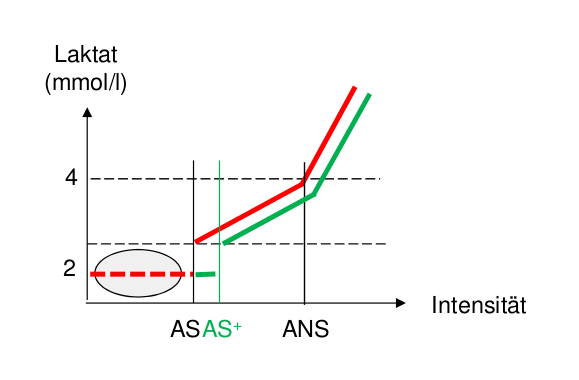
\includegraphics[width=\textwidth]{pictures/dauertraining_extensiv.png}
            \caption{Dauertraining extensiv}
          \end{subfigure}
          \begin{subfigure}[b]{0.4\textwidth}
            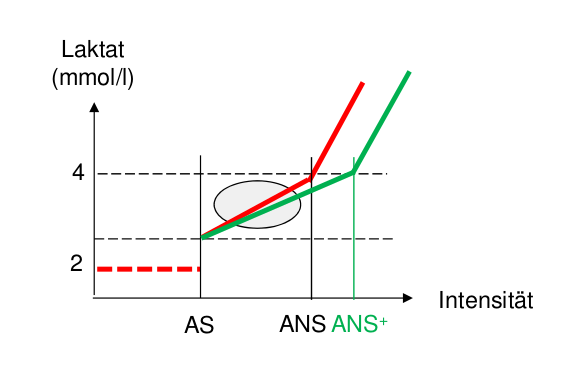
\includegraphics[width=\textwidth]{pictures/dauertraining_intensiv.png}
            \caption{Dauertraining intensiv}
          \end{subfigure}
        \end{figure}
      \item Intensiv: Intensität knapp unterhalb der ANS, Dauer \& Intensität hoch ($\leq$ ED)\\
        Intention: Rechtsverschiebung der ANS, Verbesserung des Glykose- und Laktatabbaus, Laktattoleranz (``MENTALE HÄRTE BITCH'')
    \end{itemize}
  \item Intervallmethoden: Intensität wechselnd über und unter dem ANS, durch Erholungspausen höhere Intensitäten als bei Dauermethoden mgl \\
    Intention: Verbesserung der Leistungsfähigkeit oberhalb der ANS, Phosphatstoffwechsel, hyperthrophie Herzmuskel (Belastungsphase), Erhöhung des Schlagvolumens
    \begin{figure}[H]
      \centering
      \begin{subfigure}[b]{.4\textwidth}
          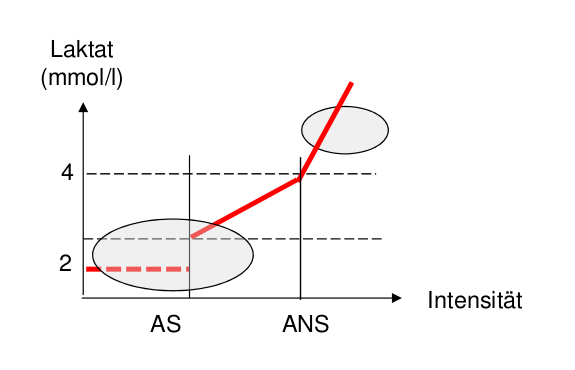
\includegraphics[width=\textwidth]{pictures/intervalltraining.png}
          \caption{Intervallmethoden}
      \end{subfigure}
      \begin{subfigure}[b]{.4\textwidth}
          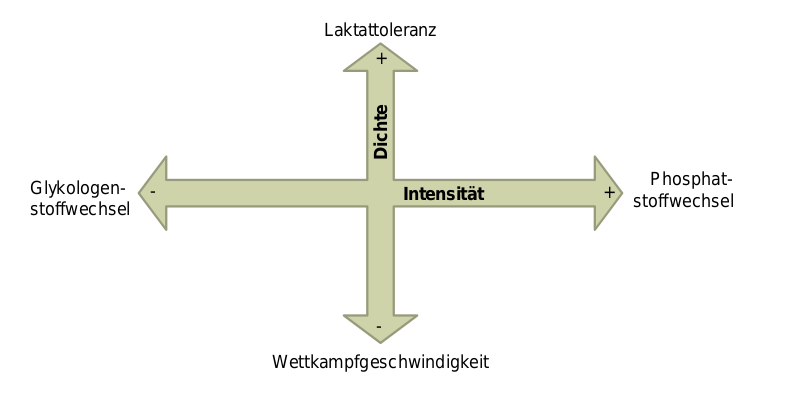
\includegraphics[width=\textwidth]{pictures/akzentuierung_der_trainingswirkung.png}
          \caption{Akzentuierung der Trainingswirkung}
      \end{subfigure}
    \end{figure}

\item Wiederholungsmethode: nahe maximale Intensität, ca. Wettkampfdauer, fast vollständige Pause\\
    Intention: Zusammenspiel aller Energiebereitstellungssysteme, alle physiologischen Prozesse
\item Wettkampfmehode: max. Intensität, mind. Wettkampfdauer, eine vollständige Pause \\
    Intention: Disziplinspezifische Belastungen, Validierung von Taktik, Trainieren der Superkompensation (d. Ausschöpfen von Reserven)\\
    Die Intensität wird beispielsweise durch Laufbandtests festgestellt, bei denen die Herzfrequenz bei erreichen der AS/ANS erreicht wird
\end{itemize}

\subsection{Trainingsinhalte}
Je nach Sportart und Leistungsziel werden andere Trainingsschwerpunkte gesetzt.
\begin{figure}[H]
    \centering
    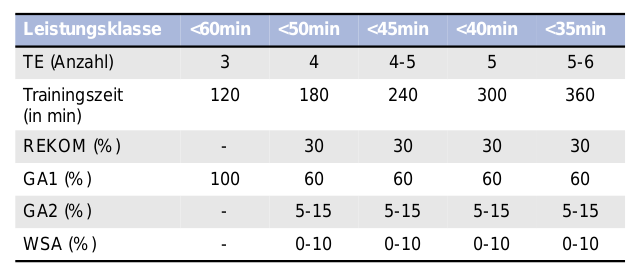
\includegraphics[width=.5\textwidth]{pictures/trainingsbeispiel_tempolauf.png}
    \caption{Trainingsbeispiel für einen Tempolauf über 10km}
\end{figure}

\subsection{Anwendung}
\begin{itemize}
    \item Leistungssport: (Ausdauer als Hauptanteil) REKOM, GA1, GA2, WSA
    \item Leistungssport (Ausdauer nicht Hauptanteil): REKOM (20min), GA1 (30-45min)
    \item Gesundheitssport: GA1 (min: 10-15min, opt: 30-45min)
\end{itemize}

Wirkungen auf die Gesundheit:
\begin{itemize}
    \item Geringere Belastung des Herzes im Alltag
    \item Höhere Resistenz für Infektion, Kälte \& Stress
    \item Positive Wirkung bei Depressionen
    \item Verbesserung der Gedächtnisleistung
    \item Erhöhter Kalorienumsatz
    \item Regulierung des Blutzucker- und Cholesterinspiegels
\end{itemize}
HIIT (High-intensity interval training) wird im Freizeitsport als unkritisch eingestuft. 
Mit HIIT können kürzere Trainingszeiten für gleiche effekte erzielt werden.

\subsection{Medizinische Empfehlung}
Sport wird ab einem Übergewicht von 20\% medizinisch empfohlen (Idealgewicht Körpergröße in cm - 100).
Das Training sollte langsam beginnen (optimal 70\% der maximalen Herzfrequenz), jedoch 10 Minuten 2-3 mal die Woche.
Bei Verbesserung der Leistung erst Häufigkeit und Belastungsumfang (jedoch nicht gleichzeitig), dann erst Intensität.

\subsection{Diagnostik}
\paragraph{Stufentest}
Der Stufentest ist ein Test für die aeroben Kapazität.
Ein Laufband wird benutzt bei dem alle 3 Minuten die Stufe erhöht wird (Anfang 60-100W, Stufe 20W).
Der Test wird abgebrochen wenn die Testperson subjektiv erschöpft ist oder eine festgelegte Geschwindigkeit erreicht wurde.
Mann misst dabei die AS und ANS mittels der Laktatkonzentration und die Geschwindikeit beim Abbruch.
\paragraph{Cooper-Test}
Der Cooper-Test testet die Ausdauerfähigkeiten einer Person.
Der Test besteht aus einem 12 Minuten Lauf bei dem die zurückgelegte Strecke gemessen wird.
Belastet werden dabei vor Allem die aerobe und anaerobe Energiebereitstellung.
\paragraph{Wingate Test}
Der Wingate Test zielt auf die anaeroben Kapazitäten ab.
Er besteht aus einem 30 Sekunden Sprint auf einem Radergometer mit konstant hohem Wiederstand.
Dabei werden die maximale Leistung, relative maximale Leistung, mittlere Leistung und Ermüdungsindex erfasst.
\paragraph{Yo-Yo-Test}
Der Test besteht aus 2x20m Lauf mit steigender Geschwindkeit, anschließend 2x5m Pause.
Der Lauf startet mit 10km/h mit einer Temposteigerung nach 8 Teilläufen um 0.5km/h.
Abgebrochen wird wenn zwei mal in Folge die Zeit nicht eingehalten.

\subsection{Zusammenfassung}
Ausdauertraining kann in jedem Alter ausgeführt werden und hat vielfältige positive Auswirkungen auf die Gesundheit.
Für optimales Training ist eine Kombination aus allgemeinem und spezifischen Methoden notwendig.
Die Grundlagen der Energiebereitstellung können eine Grundlage zum ausarbeiten eines Trainingsplans sein.
